
\subsection{De la validation à la construction des modèles de simulation par l'évaluation}
\label{ssec:evaluation_construction}

% Permanence des questions évoqués pour la construction d'un modèle de simulation, plus complexification de la validation liés à la pluriformalisation.

En montrant que la validation est dépendante au contexte, Hermann a permis de lever un certain nombre de questions remarquables par leur actualité dans le cadre de nos propre problématique de construction.  %La mise en avant d'une possibilité de validation dépendante à l'objectif nous oblige inévitablement à prendre en compte l'activité de construction comme activité validante.

\subsubsection{Des modalités de validation dépendante au contexte, l'apport d'Hermann à une première formalisation du problème}

\paragraph{Une vision de la validation différente chez les pionniers du mouvement S\&G}

Charles F. Hermann opère dans la branche des simulations appelées à l'époque par Shubik les \textit{Man-Machine Games} \autocite{Shubik1972}. Une catégorie de simulation qui intègre dans son exécution un couplage entre un ou plusieurs systèmes numériques et des humains, qui peuvent être amenés à interagir entre eux, ou avec les machines. Ce type de simulation de structure hétérogène est intéressante dans le sens où elle permet d'intégrer l'arbitraire humain dans une chaîne d'interaction complexe qui n'aurait pas pu être établie autrement, du fait de l'impossibilité de programmer des interactions et des réactions humaines face à des situations précises. Même si ce type de techniques est motivé par une multitude d'usages, ce n'est pas par hasard si elle se développe particulièrement au cours de la guerre froide aux Etats-unis, toujours sous la direction d'institutions militaires. Ce genre de techniques permettant par exemple de simuler et de reproduire des guerres au travers d'inter-relations diplomatiques et/ou économiques \autocite{Hermann1967b}, avec la possibilité de mesurer via des indicateurs adaptés l'importance et l'impact de différents scénarii sur le couple humain/machine.

Ce type de simulation est particulièrement représenté dans des publications qui traitent de la simulation au sens large, comme par exemple le journal \textit{Simulation and Gaming} ou \textit{S\&G} \autocite{Crookall2011}, dont l'activité remonte au début des années 1970. On retrouve parmi les auteurs ayant participé au développement de la discipline des personnalités importantes comme Guetzkow, Shubik, Coleman, etc. \autocite{Crookall2012}. Aujourd'hui, le terme à évolué vers ce que l'on pourrait probablement appeler des jeux sérieux, l'utilisation de l'ordinateur n'étant plus forcément un élément obligatoire dans ce type de simulation. Du côté des objectifs qui sont aujourd'hui susceptibles de motiver l'utilisation de ces techniques, \textcite{Shubik2009} définit une taxonomie en 6 objectifs : \textit{teaching, experimentation, entertainment, therapy and diagnosis, operations, training }

Cette présence d'une dimension humaine dans les simulations introduit une complexité qui touche forcément à plusieurs objets d'études des sciences humaines (psychologie, sociologie, etc.), et il n'est donc pas étonnant que l'on retrouve ce type de publication dès l'apparition des premiers ouvrages inter-disciplinaires sur la simulation, quand elle ne les pilote pas; Harold Guetzkow par exemple est un des personnages importants qui gravitent autour de Herbert Simon au GSIA (Graduate School of Industrial Administration) de Carnegie Tech dans les années 1950-56 \autocite{Guetzkow2004}, et qui a beaucoup oeuvré pour le développement de la simulation dans ces sciences politiques et psychologiques (\textit{Inter-Nation simulation laboratory}) \autocite{Janda2011, Druckman2010}. Celui ci s'inscrit exactement dans la même branche que Hermann, et apparaît deux fois comme premier éditeur dans des recueils de textes pluri-disciplinaires traitant de la simulation au sens large, preuve aussi de son implication dans le développement et la diffusion de ces techniques au delà de sa propre discipline \autocite{Guetzkow1962, Guetzkow1972}

\paragraph{L'apport du contexte dans l'évolution du sens attaché à l'activité de simulation}

Ce qui est intéressant dans ce type de simulations, c'est qu'elles forcent à penser la validation des modèles sous un angle qui doit nécessairement tenir compte de la variabilité inhérente aux comportements humains, par essence difficilement évaluables et réplicables. C'est de cette contrainte, et parce que \textcite{Hermann1967} s'intéresse aux modèles de simulation pour d'autres objectifs que la prédiction (\textit{teaching, training, theory-building}), que celui-ci développe à mon sens une vision de la validation beaucoup plus réaliste pour les sciences sociales que celle proposée à la même période par Naylor.

\foreignquote{english}{First, the validity of an operating system is affected by the purpose or use for which the game or simulation is constructed [...]}\autocite[217]{Hermann1967}

% Plus d'information à ajouter, soit sur la dite boucle (sachant que le conceptual correspond quand meme pas mal à ce que lon fait, voir Sargent2010), Si la boucle définit par les tenants de la \textit{V\&V} n'est pas inintéressante, et de façon générale résume bien le cycle de vie qui correspond à la construction d'une simulation, de nombreuses questions reste en suspens sur le choix et la mise en œuvre des techniques telles qu'elles sont décrites. La construction et la mise en oeuvre des critères en fait partie. Les objectifs sont cités dans la définitions mais on ne rentre pourtant pas dans le détail de la relation entre ces objectifs et la construction du modèle, qui est laissé à l'expertise de l'utilisateur, en cela Hermann ne propose pas mieux dans sa description d'une boucle modélisatrice que les dernières avancées portés par Sargent2010, toutefois sa réflexion est par son orientation, et par sa précocité de réflexion son intéressante il me semble à citer. les moyens technique de la mise en oeuvre par exemple ? 

%Dans l'explication sociologique, la réalité structurelle n'est pas forcément d'intérét pour la construction du modèle. (bulle)

%Cette observation amène Hermann à considérer que la validation des composantes de la structure mérite une attention tout aussi importante que la seule comparaison avec des données de sorties, notamment dans un cadre explicatif.  curl -k -o ~/backups/pinboard-backups/pinboard-$(date +\%y\%m\%d).json 'https://api.pinboard.in/v1/posts/all?&auth_token=username:APItokenhere&format=json'

En s'appuyant sur ce premier argument évoquant l'existence d'une dépendance liant processus de validation et objectif poursuivi par le modélisateur, Hermann semble \textit{de facto} mettre en défaut une définition de la simulation ayant comme première et unique vocation de représenter au mieux le système observé. Les modalités de la validation étant maintenant définies par rapport au contexte, la possibilité d'un critère unique pour juger de la validation de façon universelle paraît tout à fait improbable. Afin de montrer qu'il ne s'agit pas seulement d'une question de disponibilités des données, et pour amener par la suite sa proposition de méthode multi-critères, Hermann s'attaque donc en premier lieu à réduire la portée des confirmations apportées sur un système observé par l'emploi de la seule technique de validation basée sur la comparaison de données en sortie des modèles de simulation.

Pour montrer qu'il existe des limitations dans la confiance que l'on peut mettre dans la validation lorsqu'il s'agit de comparer des données historiques (dans le cas des simulations de reproduction de guerre, on parle ici plutôt de reproduire des séries d'événements historiques) -cela même si elles sont idéalement toute rendues disponible- aux données en sorties de simulation, \textcite{Hermann1967b} s'appuient sur les travaux de \textcite{Pool1965}.

\foreignquote{english}{This correspondence does not demonstrate that the simulation correctly represents the structure and processes that were operative in the historical occurence. We are speculating on the similarity between the historical and simulated inputs on the basis of the similarity of their outputs. Different relationships among various combination of properties in the simulation conceivably could produce outcomes like those in the historical situation.

A simulation of the 1960 national Presidential election predicted the percentage of the vote for each candidate - the outcome - with considerable success. The designers of that simulation observe, however, that \enquote{it may legitimaly be asked what in the equations accounted for this success, and whether there were parts of the equations in the simulation that contributed nothing or even did harm} Further analysis of the equations in the simulation revealed that the outcome was predicted despite the fact that at least one equation misrepresented aspects of voter turnout. Part of the structure was incorrect, but the simulated result still matched the actual outcome. Despite this difficulty, our confidence that the simulation has captured some aspects of the voting process is greater than it would have been if the simulation had failed to replicate the campaign outcome. Confidence in the simulation would increase further as the operating model demonstrated ability to produce outcomes that corresponded with various elections. In sum, the similarity between simulation and historical events can provide at best only indirect and partial evidence for the correctness of the simulated structures and processes that produced the outcome.}



Ce que nous dit Hermann ici, à la différence de Naylor, c'est que même dans le cas idéal ou toutes les données serait présente, ce mode classique de validation ne peut pas être suffisant, cela quelque soit l'objectif poursuivi par le modélisateur. Un constat que nous avions déjà acquis à la lecture des déboires des géographes avec les préceptes de validation néo-positivistes, associant dans une démarche de modélisation instrumentaliste prédiction et explication (section \ref{sssec:realite_neopositiviste}).

Ce constat reste encore valide aujourd'hui, car comme le rappelle très justement \textcite[32]{Bulle2005}, \enquote{ les problèmes posés en sciences humaines visent cependant, en général, la compréhension des phénomènes. Dans cette optique, l’objet premier de la modélisation n’est pas de faire \enquote{coïncider} les modèles construits avec la réalité qui est celle des effets. Le test par la prévision ne peut assurer des qualités explicatives des modèles.}

Un point de vue partagé par \textcite[106]{Amblard2006}, pour qui \enquote{[...] la recherche de similitudes avec les données, si elle peut être utile, ne peut absolument pas être un critère unique et définitif de validation}

Suivant ces conseil, si Forrester avait appliqué lors de la construction de son modèle \textit{Urban Dynamics} des analyses de sensibilités (voir le type de critère \textit{variable-parameter testing} de \autocite{Hermann1967}) tel que le propose Hermann, il aurait probablement conclu, comme ont pu faire ces détracteurs par la suite, à l'inutilité d'une bonne partie des hypothèses intégrés dans son modèle, qui s'avèrent en réalité très peu influente sur la dynamique observé en sortie des simulations.

Autre point important, l'existence de multiples objectifs de modélisation permet à Hermann certe de révéler la diversité et l'attachement de la validation à un contexte, mais surtout de noter d'une part comment la variation de ce dernier affecte les modalités de cette comparaison entre système simulé et système observé, et d'autre part comment cela affecte la perception du résultat engendré par cette comparaison.

\foreignquote{english}{The first comment is that the validation of an operating model cannot be separated from the purpose for which it is designed and used. [...] The second observation somewhat mediates the first. For the most part the various purposes for conducting games and simulations do not negate the need for criteria we can use to estimate the degree of fidelity with which one system (the operating model) reproduces aspects of another (the reference system). Given some purposes for using games and simulations (such as exploring nonexistent universes), finding appropriate criteria in the referent system is quite difficult. With other objectives, the value of the operating model may remain even if the fit between the model and various criteria representing the observable universe is poor (as in theory building).} \autocite[219]{Hermann1967}

Indirectement, on observe ici le transfert d'une définition de la simulation comme simple \enquote{type de modèle} vers la définition plus générale d'une simulation \enquote{ caractérisée non pas tant par l’unité d’une fonction cognitive qu’elle assurerait toujours sous une forme ou sous une autre que par son fonctionnement interne, fonctionnement qui, bien sûr, mais seulement secondairement, se trouve avoir aussi des conséquences sur sa ou ses fonctions cognitives. Une simulation nous paraît ainsi devoir être prioritairement caractérisée par ce qu’elle est – ou fait – de manière interne plutôt que par ce qu’elle fait au sens d’une fonction cognitive quelconque qu’elle assurerait toujours et qu’on en attendrait prioritairement de l’extérieur : à ce titre, nous proposons de dire qu’\textit{elle est avant tout un traitement spécifique sur des symboles et qui prend toujours la forme d'au moins deux phases distinctes. 1) une phase opératoire [...] 2) une phase d'observation [...]}} \autocite[33-34]{Varenne2013}

\paragraph{La nécessité de repenser la représentativité des modèles}

La V\&V a toujours mis en avant le fait que la modélisation soit un processus incrémental tout à fait nécessaire pour obtenir un modèle de simulation satisfaisant, que cela soit dans les analyses de Naylor, ou d'Hermann. Ce dernier se réfère dès 1967 au principe de parcimonie, une méthode qui implique une abstraction, une simplification du système à représenter, et qui pour lui met logiquement et automatiquement en péril la représentativité. \Anote{Herman_parcimonie} 

%Une parcimonie hérité du principe d'Ockham dont on sait qu'elle n'est en aucun cas un synonyme de simplicité dans sa mise en oeuvre, celle-ci nécessitant au contraire un effort intellectuel important pour déterminer quelles sont les hypothèses réellement représentatives du problèmes à analyser. %Sur le plan de complexité, Poincarré ou le prix nobel d'économie Herbert Simon à fait état plusieurs fois des capacités d'expression du complexe rendu possible par l'usage de la simulation, et cela même avec des modèles simples.\autocite{Banos2013a}

%Une description de la construction des modèles qui coincide avec ce qui a été dit auparavant sur l'importance de la nature de l'objectif poursuivie sur la perception de cette \enquote{représentativité}, et le fait que cette dernière ne fasse pas systématiquement la valeur du modèle - tant soit peu qu'on arrive à fixer une valeur - 

Dans ce que l'on comprend de l'analyse d'Hermann, la perte de représentativité attendue d'un modèle de simulation qui n'est plus strictement dirigé vers la prédiction est compensée par un gain relatif à l'objectif poursuivi qui change la nature de la validation attendue : détection d'alternatives à un comportement, mise en avant de processus simplifiés pour l'éducation, construction de théorie, etc.

Il est donc logique de voir Hermann proposer dans la suite de son analyse de repenser la notion de représentativité et la notion de validation au regard de l'objectif poursuivi par le modélisateur. Il en résulte la généralisation de cette activité de validation dont le résultat se dessine à présent sous le couvert d'un objectif et dans le jeu d'une confrontation entre deux représentations, deux construits prenant pour cible le système modélisé et le système observé. 

\foreignquote{english}{A simulation or game is the partial representation of some independent system. Usually we are interested in simulation as a means for increasing our understanding of the system it is intended to copy. Therefore, the representativeness of a simulation or game becomes extremely important in assessing its value. The process of determining how well one system replicates properties of some other system is called validation.[...] In the present analysis however, validation will be defined more broadly as any comparison between the representation of a system and specified criteria.} \autocite[216]{Hermann1967}

\subsubsection{Le problème de la validation ramené à une confrontation des représentations entre système modélisé et système observé}
\label{ssec:confrontation_sysmodelise_sysobserve}

%\hl{repetition ?}
%La question de la représentativité d'une simulation est un sujet délicat à traiter car sa valeur se dessine à l'intersection d'au moins deux activités, la construction d'un modèle opérationel et la construction d'une grille d'évaluation, deux activités dont on s'apercoit par la suite qu'elles sont en réalité étroitement liées. 

\paragraph{Quelles hypothèses pour quelle représentativité ?}
\label{p:hypothese_representativite}

Si cette \enquote{representativité} ne semble plus intervenir dans la valeur du modèle que sous une forme beaucoup plus partielle, quelle est la part de représentativité acceptable que l'on peut attendre pour qu'une hypothèse soit considérée comme explicative ? Autrement dit quelles sont les modalités qui guident l'introduction maitrisée d'une part d'empirie dans un modèle, par l'existence d'un seuil caractérisant le potentiel de représentativité à atteindre pour chaque hypothèse ? Pour l'ensemble du modèle ? 

\Anotecontent{naylor_etonnement}{On pourra peut être être étonné de retrouver la démarche de Naylor dans les approches subjectives sachant la description qu'on en a fait au préalable. Mais il y a bien une part de subjectivité dans cette démarche, l'application de chacune des étapes de la multi-stage validation faisant quand même appel à une forme d'expertise pour constituer le jeu des hypothèses que l'on estime valable en vue du test final de comparaison aux données.}

L'acceptation d'un gradient de valeur pour juger de la validation rompt avec la méthode \enquote{binaire} proposée par Naylor, la validation d'un modèle passant à présent par l'acceptation subjective d'un seuil de représentativité relatif à l'objectif poursuivi. Avec pour conséquence notable qu'une \foreignquote{english}{[...] simulation or game relatively valid for one objective may be not be equally valid for another.}

Si la notion de seuil n'est pas explicitement abordée par Hermann, c'est pourtant sous cette acceptation que la \textit{V\&V} actuelle va reprendre ce concept. Avec la position suivante, celui de se fixer un seuil de représentativité général à atteindre \textit{a priori}.

\foreignquote{english}{\textbf{Principle 2: The outcome of simulation model VV\&T should not be considered as a binary variable where the model is absolutely correct or absolutely incorrect } [...] The outcome of model VV\&T should be considered as a degree of credibility on a scale from 0 to 100, where 0 represents absolutely incorrect and 100 represents absolutely correct. 

\textbf{Principle 3: A simulation model is built with respect to the study objectives and its credibility is judged with respect to those objectives } [...] The study objectives dictate how representative the model should be. Sometimes, 60\% representation accuracy may be sufficient; sometimes, 95\% accuracy may be required depending on the importance of the decisions that will be made based on the simulation results. Therefore, model credibility must be judged with respect to the study objectives.}\autocite[15-16]{Balci1998}

La position de \textcite[166]{Sargent2010}, tout en étant relativement similaire, propose une vision plus fine et plus réaliste ou le seuil de précision attendu est attaché aux variables de sorties. Un point important sur lequel nous reviendrons plus longuement dans la suite de cette partie. \hl{ref vers la bonne partie}

\foreignquote{english}{A model should be developed for a specific purpose (or application) and its validity determined with respect to that purpose.[...] A model is considered valid for a set of experimental conditions if the model’s accuracy is within its acceptable range, which is the amount of accuracy required for the model’s intended purpose. This usually requires that the model’s output variables of interest (i.e., the model variables used in answering the questions that the model is being developed to answer) be identified and that their required amount of accuracy be specified. The amount of accuracy required should be specified prior to starting the development of the model or very early in the model development process.}\autocite[166]{Sargent2010}

\begin{figure}[h]
\begin{sidecaption}[fortoc]{ On remarquera la forte présence des techniques présentés par Hermann dans la synthèse proposé par Balci en 1986 \autocite{Balci1986}}[fig:S_syntheseBalci]
  \centering
 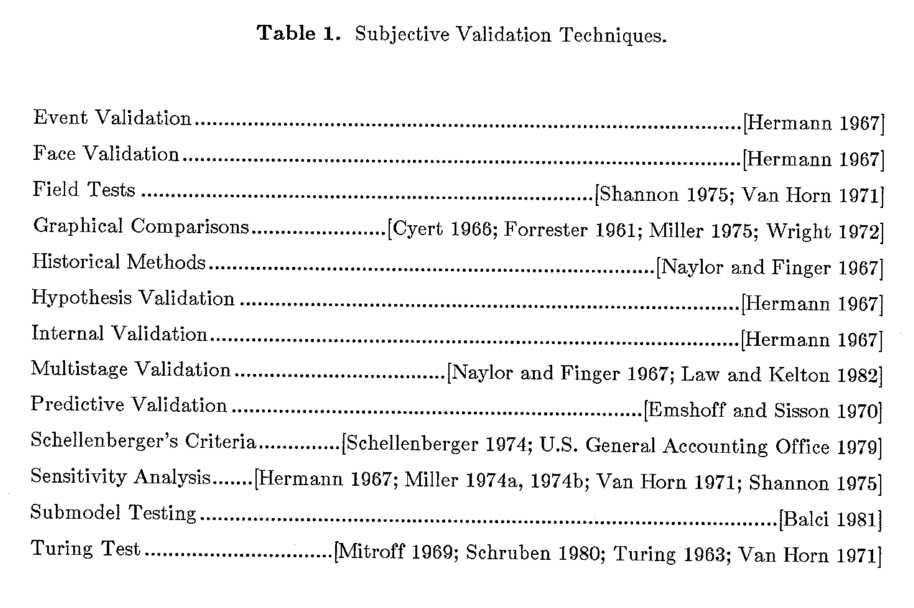
\includegraphics[width=.9\linewidth]{subjective_balci.png}
  \end{sidecaption}
\end{figure}

Ces deux citations permettent de montrer au passage comment la vision de la validation défendue par Hermann a été intégrée dans une forme très approchante par des acteurs de la \textit{V\&V} comme Balci ou Sargent, dont on a vu précédemment les définitions dans la section \ref{ssec:def_generique_validation}. Ces deux derniers sont en réalité les acteurs majeurs d'une synthèse (voir la figure \ref{fig:S_syntheseBalci}) opérée dans les années 1980-1990 \autocite{Nance2002}, dont on peut dire qu'elle est marquée par un retour à une certaine forme de neutralité (voir par exemple le rejet des aspects philosophiques décrits décrits dans la section \ref{ssec:def_generique_ validation}  qui se double d'un jargon technique spécifique à l'établissement d'un processus qualité exploitable pour l'ingénierie) . Des adaptations qui permettent probablement de mieux accepter en son sein des typologies de techniques aussi différentes que celle de Naylor\Anote{naylor_etonnement} ou Hermann. Régulièrement révisées, \textcite{Balci1998} fait ainsi état dans sa dernière taxonomie d'un catalogue de 75 techniques différentes dans lequel peuvent piocher les modélisateurs en fonction de leurs besoins. 

On se rend bien compte que dans le cadre des sciences humaines et sociales la possibilité de fixer par avance ce type de seuil n'a pas de sens, surtout dans un cadre explicatif.

%\textit{Que faut il entendre ici par partiellement ? Quels sont les leviers permettant au géographe de compenser cette perte de représentativité par un gain en compréhension sur le système à étudier ? }

Pour mieux comprendre quel est l'enjeu de cette délimitation entre un modèle réaliste et un modèle abstrait il faut évoquer cette tension permanente qui nourrit les choix du modélisateurs dans la construction d'un modèle explicatif. Deux attracteurs possibles et apparemment opposés, avec d'une part la volonté de se rattacher à une forme de réalisme au travers de l'injection d'une part maitrisée de réalité tout au long du processus de construction \Anote{durand_observation}, et d'autre part une force qui nous pousse au contraire à se détacher de cette même empirie pour ne retenir que le matériel susceptible de servir l'objectif du modèle.

La sociologue et épistémologue \textcite{Bulle2005} a bien formalisé ce dilemme dans la nécessité pour tout modélisateur de positionner son modèle sur un gradient opposant le réalisme des causes des modèles explicatifs \Anote{bulle_modele_explicatif}, au réalisme des effets des modèles descriptifs. 

Pour mieux comprendre quelles connaissances peut-on attendre d'un tel positionnement sur ce gradient, le mieux est encore de commencer par évoquer un de ses extrêmes, en invoquant par exemple le modèle universellement connu de Schelling. De par sa portée d'application extrêmement générale et la nature très abstraite de ses paramètres celui-ci constitue en soi un extrême intéressant pour comprendre où se situe encore l'explication lorsque le détachement de la réalité est à ce point éloigné. Sur ce point, les analyses de \textcite{Bulle2005} et \textcite{Phan2008, Phan2010} se réfèrent principalement à l'essai de \textcite{Sugden2002} pour évoquer quels types de relations entre les deux mondes peut on attendre de ce type de modèle épuré. 

Les résultats qui dérivent de la mise en dynamique des règles dans le modèle de Schelling sont d'une telle universalité, d'une telle robustesse qu'il n'est plus question de confronter les résultats ainsi obtenus à la réalité. A cet égard le potentiel explicatif de ce type de modèle s'oppose selon \textcite{Bulle2005} à tout réalisme empirique. De ce point de vue, \enquote{le modèle n'est pas tant une abstraction de la réalité qu’une réalité parallèle [...] bien que le monde du modèle soit plus simple que le monde réel, celui-ci n'est pas une simplification de l'autre. Le modèle est réaliste dans le même sens qu'un roman peut être appelé réaliste [...] les personnages et les lieux sont imaginaires, mais l'auteur doit nous convaincre qu'ils sont crédibles } \autocites[131]{Sugden2002}[10]{Phan2008}

L'effet d'une telle recombinaison d'hypothèses revient à mettre en oeuvre un \enquote{monde crédible} où l'inférence inductive est mobilisée pour identifier des similitudes significatives entre les deux mondes. \autocites{Livet2006, Phan2008}. Tout le travail réside donc dans l'interprétation prudente qui peut être faite entre ces résultats d'un monde factice et d'une réalité.

Un processus commun utilisé dans toute oeuvre de fiction pour piquer la curiosité de l'observateur, la mise en exergue volontaire d'une tendance du monde réel dans un monde imaginaire permettant d'entamer une réflexion sur l'existence, la portée, la nature de cette même tendance dans le monde réel. Les villes ou les sociétés mis en avant dans des oeuvres de fiction cinéma ou dans la littérature ne sont jamais que des mondes plus ou moins crédibles (Gotham City, 1984, Matrix, la série Black Mirror, etc. car la liste est longue ...)  pour mettre en avant un discours, ou des tendances du monde réel sur lequel doit porter le questionnement; (http://www.influxpress.com/imaginary-cities/ , \href{http://cybergeo.revues.org/1170#tocto1n9?}{cybergeo})

Si le discours scientifique n'a clairement pas cette obligation ludique, il n'en reste pas moins que ce processus de reconstruction crédible est déjà un outil formidable pour questionner les processus à l'oeuvre dans le monde réel \Anote{ruffat_samuel_ville}. Mais cette ambiguïté de lecture a déjà mené à de nombreux malentendus, d'une part envers le grand public (Voir forrester, mais également \Anote{deffuant_debat}) qui pourrait prendre des résultats de simulation pour la réalité avec tout les conséquences que cela suppose, mais également parfois entre scientifiques provenant de divers horizons. Ainsi après la lecture de la critique par \textcite{Chattoe2011} de l'article de \textcite{Yanoff2009}, il ressort toute la difficulté d'évaluer la méthodologie et le travail réalisé autour d'un modèle au travers d'une seule publication, notamment lorsque la fonction cognitive recherchée par les modélisateurs n'est pas décrite explicitement, ce qui provoque aussi ce décalage entre attente du lecteur et le processus réel de recherche qui sous-tend la construction du modèle. \hl{dp: TROP ALLUSIF}

\textit{Doit on se contenter de ce seul mode explicatif ? Existe t il un moyen pour renforcer la confiance dans la capacité explicative des hypothèses ainsi mobilisés ? } 

%% DEBUT - EN ATTENTE DE LA REPONSE DE VARENNE %%

\textcite{Bulle2005} evoque bien l'existence de modèle à cheval entre potentialité explicative et potentialité descriptive. Ainsi \enquote{appliquée aux processus sociaux réels, la simulation peut allier au potentiel descriptif offert par l’imitation d’effets empiriquement observables, le potentiel explicatif que lui confère la mise en œuvre de relations causales effectives. }

A la différence de modèles trop simples qui n'offrent que de maigres accroches avec la réalité, c'est donc par la réintroduction maitrisée de l'empirie dans les modèles de simulation construits que l'on peut espérer la mise en route progressive d'un processus de validation.

Seulement conformément au type de problèmes que l'on a déjà pu effleurer en traitant de philosophie des sciences dans la section \ref{sssec:philo_sciences}, le processus de validation se heurte rapidement à la différence de nature entre les résultats produits par des hypothèses \textit{reconstruites} et le monde réel. Tout comme le substrat est artificiel, le résultat produit par cette dynamique reste le produit d'un monde reconstruit -in silico- L'existence de ce nouveau niveau d'empirie amène les épistémologues comme Varenne à parler ici d'\enquote{expérience concretes du second genre} faisant alors de la simulation une \enquote{quasi-expérimentation} \autocites{Varenne2001, Varenne2007, Phan2008}

On en déduit que quelque soit notre placement sur ce gradient, il est effectivement vain de chercher à valider un modèle en usant d'un quelconque \enquote{seuil de suffisance} caractérisant \enquote{l'injection de réalisme à atteindre qui autoriserait une inférence certaine sur le monde réel}, puisque de toute façon cette inférence s'appuie sur un résultat \enquote{artificiel} forcément discutable. \Anote{bulle_modele_autonome} \Anote{phan_livet_modele} 

La démonstration précédente nous indique plusieurs pistes de réflexions.

D'une part l'objectif de réalisation d'un modèle au réalisme uniquement structurel n'a pas de sens, même avec beaucoup d'hypothèses, car elle ne permet en aucun cas de garantir la justesse d'une comparaison entre données empiriques et simulés, et n'offre donc aucun critère d'arrêt pertinent dans l'activité de modélisation.

D'autre part à moins de retomber dans les débats philosophiques évoqués dans la section \hl{xxx}, elle nous oblige à penser le modèle pour ce qu'il est vraiment, non pas une construction guidée par la validation, mais la construction d'un raisonnement appuyé par une simplification orienté par et pour un but. Peu importe alors le fait qu'une divergence s'installe entre le monde tel qu'on l'observe et le système modélisé, au contraire.

\foreignquote{english}{In all probability some distributions of events or some kinds of hypotheses will produce results with unacceptable divergence between the operating model and the observable universe. Although these incongruous may not pinpoint the inadequacy in the model, they should provide a diagnosis of the general area which seems unrepresentative.} \autocite[226]{Herman1967}

Mais ce terme de \enquote{simplification} souvent employé reste d'emploi ambigue, la modélisation nécessitant comme le dit \textcite{Haggett1965} non pas tant la mise en oeuvre d'une simplification aveugle, qu'une idéalisation guidé par la volonté de mettre à nu des propriétés du système observé. \textcite{Brunet2000}, pour qui la modélisation est également un processus de recherche, propose même pour éviter toute confusion sur les termes de dénuder la définition de modèle de cette fausse directivité, le modèle devenant dans sa version la plus épurée une \enquote{représentation formalisée d'un phénomène}; le terme \enquote{représentation} intégrant alors toute la complexité sous jacente à une telle formalisation : \enquote{Il va de soi que cette représentation passe par plusieurs filtres, qui tous tendent des pièges : la perception du phénomène, sa représentation, la construction d'un modèle, l'interprétation du sens de ce modèle et la capacité du modèle à rendre compte du phénomène.}

Un point de vue semble t il partagé par Varenne pour qui le terme simplification est  \endquote{[...] un glissement d’attribution indu. Puisque l’usage du modèle est relatif (à un observateur et à un questionnement), on ne peut dire que le modèle doit être un objet simple en lui-même ou dans l’absolu. Il convient donc de regarder sous quel aspect exactement il doit apparaître simplificateur, sous quel aspect il devient un outil facilitateur, un outil de facilitation.}

Dès lors, {[...] on comprend déjà qu’un modèle n’est pas ce qui est recherché en tant que tel, mais ce qui facilite la recherche d’information au sujet d’un système réel ou fictif, cela dans le cadre d’un processus à visée de représentation, de connaissance, de conceptualisation, de conception ou encore de transformation. Il est le moyen plus que la fin. C’est pourquoi je m’aventurerai, à partir de maintenant, à user plutôt du terme de facilitation que de celui de simplification [...]} (voir également la section \ref{ssec:rapell_termes_generiques}) \autocite{Varenne2008}

Comme déjà évoqué par les géographes, ce n'est pas tant \enquote{le modèle} que ce qu'il y a \enquote{dans le modèle} qui nous intéresse \autocites{Sanders2000, Besse2000}, et il faut rajouter par là même aussi l'histoire justifiant de cette configuration. 

Reste alors à explorer comment cette \enquote{facilitation} s'exprime au travers de la construction du modèle de simulation. Seulement comment analyser la pertinence d'une représentation prise en dehors de son contexte, les choix intervenant lors d'une modélisation ne répondant pas à une logique universelle pré-établie, étant comme on l'a vu motivé et modifié par un (ou plusieurs) objectif. Varenne a identifié une vingtaine de ces fonctions de facilité de médiation pouvant motivé la construction ou l'utilisation générale d'un modèle. Or il me semble qu'une fois rapporté au modèle, on est bien obligé de constater l'impact que peut avoir cette diversité d'objectifs dans le choix menant à différentes représentation d'une même hypothèse dans le modèle. Etait-ce pour dénoter une entité réelle (un agent = un individu, une ville, une innovation ) ? Est ce dans le but de simplifier pour la compréhension ? pour les performances ? pour répondre au principe de parcimonie ? Ou les trois à la fois ? (une population agents homogène devenant une equation de croissance par exemple ) Etait-ce un choix fait à la suite parmi une multitudes d'autre essais (différentes équations plus ou moins représentative du phénomène à considérer) ? etc. Il n'y a aucune raison pour que les mécanismes intégrés aux modèles soit homogènes. Dans le cas d'un modèle de migration inter-ville, il est en effet plus intéressant de mobiliser les populations de façon aggrégé si on s'intéresse aux règles intervenant dans la dynamique d'interactions entre les villes, par contre, si il s'agit d'observer l'impact que peuvent avoir des règles de comportements sur ces interactions, ce niveau peut devenir pertinent; cette aproche ne chassant évidemment pas la première, au contraire les couplages étant bienvenu. Normalement tout ces choix devrait être explicité, ce qui est rarement le cas, vu la complexité d'une tâche qui apelle pour être sérieuse l'analyse d'une activité de raisonement accompagnant le modèle dont les jalons de reflexion ont bien souvent disparu. \autocite{Varenne2013b}

La tendance à la pluriformalisation \Anote{pluriformaliser} permise par les modèles multi-agent ne vient pas non plus faciliter cette tâche, car ces modèles de simulation qui peuvent déjà intégrer -et c'est d'ailleur pour cela qu'ils ont autant de succès- sans problème une hétérogénéité d'échelle, de niveau d'abstraction, de modèles, doivent aussi compter avec l'intégration de formalismes mobilisant des temporalités et/ou des échelles différentes \autocites{Varenne2008,Varenne2012a}. Ces couplages n'étant pas toujours évident, y compris au niveau informatique ou des artefacts, c'est à dire l'apparition de mécanismes non prévu et difficile à expliquer d'un point de vue purement théorique, peuvent venir rapidement venir perturber les belles ontologies réalisés en amont. 

Même les modélisateurs ont parfois du mal à s'y retrouver, par exemple il n'est pas toujours évident d'expliquer pourquoi on a choisit de coupler pour certain mécanismes le formalisme agents avec celui des équation différentielle ? Il faut alors comprendre que dans certains cas, c'est aussi ce qui a pu motiver le modèle, l'intérét de la pluriformalisation étant justement ce qu'il faut démontrer en comparaisons des approches traditionnelles prisent séparement. Plusieurs réflexions ont montré qu'il s'agissait d'un type de modélisation en devenir et en voie de démocratisation, les formalismes pour la simulation informatiques (multi-agents, micro-simulation, ac) ou mathématiques (systèmes dynamiques) utilisés n'ayant jamais eu vocation à s'opposer (approche individu - centré contre approche mathématique traditionnelle) comme on aimerait parfois nous le faire croire \autocites{Sanders2013, Banos2013}. 

%% FIN - EN ATTENTE DE LA REPONSE DE VARENNE %%

Une façon de dépasser cette problématique de la validation est d'accepter le fait que le réalisme des hypothèses ne soit plus vraiment un objectif, mais plutôt la réalisation conséquente d'une expertise qui tient essentiellement de l'angle théorique choisi pour éclairer un problème.

Autrement dit, la confiance établie dans les capacités explicatives des hypothèses choisies ne se juge pas tant dans la comparaison des résultats attendus avec le réel observé, que dans l'exploration du monde crédible ainsi simulé en fonction de critères experts construit sur une observation du réel, dans l'espoir d'en dégager une connaissance qui doit encore être vérifiée \Anote{denise_geopoint}. 

Le problème est ici en quelque sorte inversé, ce n'est plus une qualification directe du réel qui est visé par le modèle, mais le modèle qui est visée par notre compréhension du réel au travers de critères experts. Ceux-ci viennent questionner et mettre en tension ce monde virtuel en lui imposant de nouvelles contraintes, révélant par là même les forces et les faiblesses de nos hypothèses dans le modèle. On oppose dans la construction du modèle un jeu d'hypothèses susceptible de produire des résultats attendus, à la réalité des conclusions apportés par la mise en oeuvre effective d'une dynamique que l'on contraint volontairement.

A ce titre, et en s'inspirant de la remarque faites par \textcite{Bulle2005} à ce sujet, il sera toujours nécessaire et légitime de questionner la pertinence des rapports mesurés entre les liens causaux proposés dans le modèle et le ou les critères qui sont censés en rendre compte.

On retrouve ces réflexion dans les termes de \enquote{validation interne} et \enquote{validation externe} introduit par \autocite{Amblard2006}, qui est un des rares publications abordant de façon assez précise le passage d'une \enquote{validation} à une \enquote{évaluation} des modèles de simulations en sciences humaines et sociales. La relation d'inter-dépendance entre validation interne et validation externe y est clairement exposé, à travers l'impact des analyses de sensibilités sur la structuration des modèles, et l'exploration des classes de comportements émergentes observés, les deux se rapportant au final à une comparaison faisant intervenir des critères d'évaluation, des fait stylisés ou des données.

\enquote{L'analyse de sensibilité, si elle peut s'appliquer pour tester la robustesse des résultats d'un modèle, peut également être utilisée pour tester la robustesse de la structure du modèle. En modifiant les hypothèses réalisées dans le modèle, par exemple en modifiant les structures organisationnelles, le modélisateur obtient des indices relatifs à la stabilité de son modèle et de ses hypothèses. Ces indices lui permettent précisément de jauger l'importance du choix d’une hypothèse et l’influence de son remplacement par une autre sur un aspect particulier du modèle. [...] Une autre propriété importante qu'il s'agit d'étudier au cours de cette étape de validation interne, concerne les classes de comportements produites par le modèle. Les simulations multi-agents produisent ce qui est assez communément appelé des « comportements
émergents » (voir chapitres 14, 16 et 17), c'est-à-dire des comportements qui ne sont pas exprimables en utilisant uniquement les hypothèses réalisées sur les comportements individuels}. Deux propriétés qui font ainsi écho à une méthode de la validation externe qui \enquote{[...] consiste à rapprocher les classes de comportements (identifiées lors de la validation interne) à des comportements saillants du système-cible : les faits stylisés. Ce rapprochement, s’il peut être fait avec des faits stylisés identifiés a posteriori (permettant par exemple de découvrir dans les phénomènes empiriques, des comportements stylisés qui auraient pu passer inaperçus), possède, on le sent bien, plus de force lorsque les faits stylisés sont déterminés avant même la modélisation comme des comportements que l'on cherche à reproduire par le modèle ou dont on se servira comme un critère de validation parmi d'autres (rétrodiction).}

Ces deux points nous incite ainsi à pratiquer une évaluation à contrepied de la démarche habituelle, alternant validation interne, puis externe. On met alors de coté un instant la validation interne comme exploration non dirigé des comportements du modèle pour se concentrer sur une exploration, moins complète, ou c'est le désir de rapprochement qui vient piloter cette fois ci l'exploration des comportements. Les modélisateurs peuvent en effet introduire les hypothèses dans un modèle de simulation dans le but de satisfaire, ou \textbf{de ne pas satisfaire} ces critères. En effet on a bien précisé que l'objectif de correspondance avec les données n'était plus la priorité dans l'établissement de tels modèles de compréhension, sinon pourquoi ne pas se contenter d'un modèle de Gibrat pour expliquer la hierarchies des systèmes de villes ? 

Autrement dit, il s'agit de mobiliser de façon volontaire cette tension entre hypothèses du modèle et critères d'évaluations mis en place pour en rendre compte afin de savoir si oui ou non cette question valait la peine d'être posé. Reste qu'il faut avoir les moyens techniques de pouvoir répondre à cette question. % Avant de revenir à cela, question de la proof of possibility, impossibility

Il semble que cette mise en tension se satisfait assez bien d'un cadre d'analyse basé sur l'activité de modélisation, ou les critères et les hypothèses, et c'est bien pour cela que l'on mobilise la simulation, ne sont pas tous nécessairement connu à l'avance. Ce qui laisse la place au cours de cette confrontation à l'avénement d'une certaine surprise, à même de produire une connaissance, et de guider le choix des modélisateurs à chaque nouvelle étape du modèle. 

% Les critères toutefois entretiennent un lien avec les hypothèses dont ils sont censé rendre compte, on peut donc imaginer que la parcimonie exprimé dans la construction des modèles puisse faire en lien des critères porteurs de cette connaissance exprimés sur le comportement du modèle. 

% Une remarque d'autant plus valable lorsque on sais que cette histoire se construit en confrontation avec la construction et la mise en oeuvre progressive des critères constitutif du système ciblé.

% Ce qui pose effectivement toujours la question de la nature des connaissances attendues dans une telle perspective.

\paragraph{L'abduction, un phénomène clef moteur dans l'activité de modélisation}

La présence d'une hypothèse dans le modèle se justifie donc tout à la fois par l'expertise du modélisateur que par son adéquation, ou sa non adéquation \textbf{potentielle} avec différents critères de validation. La subjectivité de l'expérimentateur joue sur les deux tableau, et donne à voir dans cette subtile inter-dépendance qui relie le choix des hypothèses et le choix des critères une forme incertitude quand au résultat assez difficile à prévoir et quantifier.

Que se passe-t-il lorsque le potentiel explicatif d'une hypothèse pourtant appuyé par des résultats empirique constaté dans le système observé s'avére invalidé par une analyse de sensibilité ou un critère d'évaluation ? Et cela, alors même que l'experimentateur considère celle-ci comme étant indispensable dans le développement d'une dynamique donné ? Que se passe-t-il au contrare lorsqu'un critère d'évaluation est atteint alors que cela n'était pas attendu au vu de la structure du modèle ? 

%La fonction heuristique de la simulation pouvant s'exprimer tout autant dans cette \enquote{surprise} d'une divergence entre le potentiel investit dans les hypothèses et les critères selectionnés, que dans la surprise suivant l'introduction de nouveaux critères contraignant le modèle, et remettant en cause ce même potentiel de représentation investit dans certaines hypothèses. 

Il y a une divergence nécessaire entre la volonté du modélisateur de rendre compte d'un système observé par un réseau d'hypothèse qui lui parait parcimonieux, nécessaire et cohérent d'un point de vue thématique (le potentiel investit), et la réponse effective apporté par la mise en dynamique de ces causalités lues au travers des critères selectionnés pour en rendre compte. % la possibilité d'infirmer ou d'affirmer de nouvelle connaissances, avec le développement de nouveaux critères, de nouvelles hypothèses ayant jusque là échappé aux raisonnement du modélisateur.

\foreignquote{english}{In developing a game or simulation, the designer is required to be explicit about the nature and relationships between the units in the operating system and their counterparts in the observable universe. He must specify the conditions which cause a relationship to vary. In constructing an operating model a connection between previously unrelated findings may be discovered. Alternatively, a specific gap in knowledge my be pinpointed and hypotheses required by the model my be advanced to provide an explanation.} \autocite[219]{Hermann1967}

La surprise volontaire ou involontairement produite au cours de cette divergence, et qui accompagne généralement l'activité de modélisation, revient sous le nom d'abduction, le terme venant de Charles S. Peirce \autocites{Besse2000, Banos2013, Phan2006, Livet2014} 

Une capacité dont on a déjà vu en citant Hacking \autocites{Hacking1983,Hacking2003, Hacking2006} qu'elle tenait plus d'une propriété inhérente à l'humain, existant de façon préalable à ses créateurs Aristote, ou Peirce. Un modèle de cognition remis au gout du jour ces dernières années, et qui parait correspondre assez bien, est celui du \enquote{cerveau statisticien},  \enquote{cerveau prédictif}, ou \enquote{cerveau bayésien} pour qui \enquote{penser c'est avant tout prédire}. Cette machine à inférer permanente, construisant des logiques qui lui sont propre à partir du peu d'informations qui lui sont donnés directement ou indirectement, quitte à rapeller en urgence d'ancien schéma, fournit comme on pourrait s'en douter plus de mauvaises prédictions que de bonnes. Mais peu importe, ce qui est important ici, c'est sa capacité à apprend rapidement de ces erreurs. 
%Cette logique bayésienne qui consiste à formuler une hypothèse a priori de façon consciente ou inconsciente \Anote{kauffman}, prise de façon rapide ou lente, basé sur nos connaissances passés ou sur notre environnement présent, pour la confronter et la réévaluer au yeux de la réalité de façon itérative correspond assez bien il me semble à ce que l'on pourrait apeller \enquote{abduction}, apellée également \enquote{inférence de la meilleure explication}. 
Ainsi pour Stanislas Dehaene, partisant de ce modèle cognitif, \enquote{Ce que Pierce appelle l'abduction n'est rien d'autre que ce que les sciences cognitives contemporaines nomme l'inférence bayésienne et qui consiste à mener un raisonnement probabiliste en sens inverse afin de remonter aux causes cachées d'une série d'observations.}

Cette théories qui touche à l'ensemble des disciplines oeuvrant dans le champs des sciences cognitives sont mieux décrites par exemple par Stanislas Dehaene dont les cours sont disponibles sur le \href{http://www.college-de-france.fr/site/stanislas-dehaene}{@site} du Collège de France. Toutefois dans l'utilisation des modèles de simulation d'une part ce n'est pas le monde réel qui nous surprend, mais ce qui se passe dans le modèle de simulation, et d'autre part il est plus intéressant d'adopter une démarche active et créative dans la mobilisation des hypothèses, afin de maximiser la surprise plutot que de la miminiser, de dépasser son horizon de connaissance plutot que de s'y conforter. 

% Proof of possibility ? 
Comme le résume bien Banos dans son HDR, \enquote{l’esprit même de l’abduction au sens de Peirce, désignant cette capacité de l’être humain à générer des hypothèses temporaires à partir de l’information incomplète dont il dispose. Appliquée à la démarche scientifique, l’abduction renvoie ainsi à la capacité du scientifique à se mettre en position d’étonnement, à se laisser guider par la recherche de l’inattendu et plus généralement à laisser libre cours à sa créativité.} \autocite{Banos2013}

Comme on pouvait alors si attendre, les motifs développés par les modélisateurs soutenant cette approche sont très loin de ceux attendus pour la prédiction, ou c'est d'abord la robustesse des résultats qui prime, car \enquote{[...] dans le cas d’une modélisation compréhensive, où l’objectif est d’apprendre des propriétés du système que l’on reconstruit \textit{in silico}, le fait d’avoir, pour une partie des conditions expérimentales des comportements très erratiques du système, loin de discréditer le modèle nous apprend au contraire des éléments de son fonctionnement et nous permet même d’anticiper le fonctionnement du phénomène modélisé. Si sous certaines conditions le modèle est très instable c’est une information très enrichissante sur le modèle et sur le phénomène considéré.} \autocite{Amblard2010} 

Force aussi de constater que cette incrémentalité dans la construction d'un modèle de simulation ne suit pas vraiment un modèle linéaire de développement, et s'accompagne, au moins dans les sciences humaines et sociales d'une activité de raisonnement en partie imprévisible. Ainsi il peut paraitre paradoxal pour un modélisateur débutant de voir à quel point il est important de \enquote{malmener} les modèles que l'on a précédemment construit avec raison et parcimonie. L'important ici nous dit \textcite{Amblard2010}, c'est que cela participe à l'élaboration de la compréhension ou de l'explication des phénomènes considérés. Car comme le dit dans son tout premier principe \textcite[65]{Banos2013}, modéliser c'est avant tout apprendre.

D'autre définitions de l'abduction \Anote{abduction_definitions} permettent de mettre en valeur d'autres de ces propriétés, la création en est une, mais avec celle-ci vient aussi la selection. Si on se rapporte aux processus de cognition, la conscience apparaitrait par exemple comme un filtre discrétisant, selectif, d'une pensée inconsciente fluctuante et résolument continue. On peux supposer que lors de la modélisation, ce type de processus est également à l'oeuvre, et il n'est pas rare lorsqu'on construit un modèle de simulation d'avoir à choisir, ou à ne pas choisir, avec plusieurs hypothèses ou implémentation d'hypothèses alternatives. Le deuxième choix expliquant aussi en partie pourquoi les interfaces utilisateurs de nombreux modèles de simulation Netlogo sont aussi riches en boutons de selection.

%Cela soulève la possibilité d'hypothèse explicative concurrente ou inter-dépendante dans l'apparition d'un phénomène, dont certaine échappe forcément au seul modélisateur géographe du fait par exemple de la nature inter-disciplinaire des objets engagés, auquel il faut encore appliquer une selection plus consciente en décidant de mettre plus ou moins en avant des hypothèses susceptible de surprise. 

%La surprise ne vient donc pas seulement du modèle, mais aussi de ce que font les autres manipulant les modèles, surtout dans le contexte inter-disciplinaire ou nous évoluons, les limites de nos connaissances se manifestant assez vite lorsqu'il s'agit d'étudier un phénomène ou un objet partagé, comme les villes par exemple. 


%% A REPLACER

% S'exprime dans une dynamique ? 
\paragraph{Quels critères d'évaluation pour quelle mesure des hypothèses ?}

On a montré que l'objectif d'une adéquation avec le système observé n'avait pas de sens, mais on n'a pas évoqué les modalités de ce rapprochement dans le rapport d'évaluation existant entre hypothèses et critères quantitatif mobilisés dans le modèle. Pourquoi ne pas envisager ici une validation externe basé sur une comparaison empirique et terme à terme des hypothèses constitutive entrant dans la structure causale du modèle  ?

Pour \textcite{Batty2001} et du fait l'\textit{Observational Dilemna}, cette solution n'apparait pas faisable en général. \foreignquote{english}{In principle, each element of this process should be explicit and should be capable of being validated with observed data. In practice, this is rarely if ever the case. The data set would be too large, it would be impossible to collect in its entirety, it may be impossible to even observe and measure. Yet the processes are known to be important. Other criteria must thus be used.} Outre donc la question de la disponibilités des données en sciences humaines et sociales, l'\textit{Observational Dilemna} démontre l'impossibilité de s'abstraire de cette intrication entre cause et effet lorsqu'on observe un phénomène (complexe) en sciences humaines et sociales. De fait, cette caractéristique des systèmes complexes suppose aussi l'impossibilité d'établir l'unicité des hypothèses avancées pour décrire un phénomène, mais aussi par extension celle des critères d'évaluation, qui reste eux aussi des construits formulés sur la base d'une observation du système observé.

On peut ajouter à çà une autre limite concernant les données, on a effet vu que toutes les hypothèses du modèles n'avait aucune raison de se placer au même niveau d'abstraction, ou d'appartenir au même formalisme. Il est par exemple déjà difficile d'accéder à des données dans une fenêtre spatio-temporelle donné, est-il possible d'en avoir sur plusieurs fenetres, voire plusieurs fenetres simultanées ? 

Pour \autocite{Amblard2006}, si cette validation externe basé sur une comparaison quantitative avec les données n'est pas impossible, elle n'en reste pas moins difficile à mettre en oeuvre de façon systématique, pour les raisons évoqué ci-dessus, l'appel à des critères d'évaluation plus qualitatif, dont il faut déjà justifier la construction, restent les plus évidents à mettre en oeuvre. Un point de vue assez logiquement partagé par \textcite{Batty2001} \foreignquote{english}{ [...] complex systems models have multiple causes which display a heterogeneity of processes that are impossible to observe in their entirety. The focus is on more qualitative evaluation of a model’s plausibility in ways that relate to prior analysis of the model’s structure.} 

% A deplacer et a remettre dans le flux au desssus ? 

Une des autres originalité dans l'analyse d'Hermann réside dans les remarques très juste et très précoce qu'il a formulé sur la relativité des hypothèses et des critères mobilisé dans les modèles. Celui-ci est en effet tout à fait conscient qu'il ne s'agit pour l'une comme pour l'autre que d'assertions sur la réalité, comme nous l'avons déjà discuté auparavant. Il propose donc d'essayer de faire au mieux. En adoptant une validation multi-critère \Anote{methode_hermann} intégrant les objectifs ayant guidé la construction du modèle il espère ainsi renforcer le crédit qu'il est possible d'apporter aux simulations. \foreignquote{english}{We have arrived at the position, then, that multiple validity criteria are needed because of the error of measurement and because of the recognition that criteria can be only assertions about \enquote{reality}} 

Comme on pouvait toutefois s'y attendre, cette impossibilité d'admettre l'unicité des critères pour juger la structure causale mobilisé s'insère dans un questionnement plus large. Faut-il effectivement juger la valeur des hypothèses constituantes de cette structure uniquement vis à vis de la réponse à ces critères ?

Si on en croit \textcite[17]{Besse2000}, pas vraiment, car cela serait oublier qu'\enquote{Une hypothèse possède une signification propre, avant même d’avoir été engagée dans l’aventure hautement improbable des programmes de validation. Cela nous conduit à reconnaître dans l’activité scientifique un moment de la production du sens, a coté du mouvement vers l’établissement des vérités.}

L'abduction de part l'argument naturaliste évolutionniste qu'on lui prête,dépasse le simple cadre de la logique dans lequel de toute façon elle posait déjà problème, et n'intervient donc pas comme un moyen de preuve : \enquote{ On nous propose plutot d’envisager l’ensemble des démarches par lesquelles les chercheurs s’orientent vers les hypothèses qui semblent plausibles, en éliminant celles qui ne peuvent etre considérées comme pertinance. } A ce titre, \enquote{La démarche abductive permet un authentique gain de sens, une progression dans l’élucidation}

Un argument supplémentaire pour parler d'évaluation plutôt que de validation \autocite{Amblard2006}, car celle-ci s'inscrit dans un projet parallèle à l'activité de construction du modèle, dont la mise en œuvre implique sinon la construction au moins l'existence préalable d'hypothèses, et d'indicateurs pertinents sur le système observé; une expertise cumulé qui dépasse de loin en durée et en travail le seul projet de construction d'un modèle, et fait souvent intervenir un système de modèle dans une démarche de construction des connaissances de portée beaucoup plus large que cette seule construction de modèles de simulation. Un point que l'on a déjà abordé dans le paragraphe \ref{decorreler_validation} pour justifier d'une décorrélation des problématiques de la Validation vue sous l'angle réducteur de cette seule activité de modélisation multi-agents.

Que cela soit les paramètres, valeur de paramètres, hypothèses mobilisés, choix d'implémentation des hypothèses, critères d'évaluations ( fait stylisés ou données ) construit ou choisi, tout ces étapes ne peuvent être mis en oeuvre si on n'accepte pas de voir l'activité de modélisation pour la simulation comme parti prenante d'une activité de construction des connaissances plus globales. C'est ce qui rend aussi difficile l'évaluation de publication soutenant l'originalité d'un modèle de simulation par un public n'ayant pas connaissance de ce système de modèles et des interactions complexes et réflexives qui relient ceux ci, que cela soit en amont ou en parallèle de la construction des modèles de simulations.

Cette démarche globale a été plusieurs fois théorisé par les géographes \autocites{Besse2000, Sanders2000, Mathian2014}, et une application plus explicite des relations que peut entretenir un modèle de simulation avec d'autres type de modélisation (statistique, spatiales) peut être vu dans la thèse de Clémentine Cottineau \autocite{Cottineau2014a, Cottineau2014b}. 

De plus, il reste difficile donc d'éliminer une hypothèse présente dans le modèle en fonction de sa seule mise en défaut observés à un instant $t$ donné dans la construction d'un modèle, notamment lorsque la présence de celle ci fait sens du point de vue des objectifs qui ont été fixés par le modélisateur. 

D'autant plus qu'il faut aussi prendre en compte cette double dynamique dans lequel opère la construction et la complexification des modèles et des indicateurs pour en rendre compte. Une hypothèse valable à un instant $t$ ne le sera peut etre plus à un instant $t + 1$, ou inversement. 

Peut être n'était-ce simplement pas le moment pour intégrer cette hypothèse au modèle, celui-ci étant encore trop simple ? Peut être manquait-il des interactions pour que sa dynamique soit révélé ? Peut être que l'indicateur devant rendre compte de cette dynamique n'est pas adapté ? Peut être que l'implémentation proposé n'était tout simplement pas la plus adapté à ce moment là ? etc. 

Ce qui a mon sens soulève ici plusieurs remarques : 
- il est vraiment difficile de savoir ce qui va se passer avec l'intégration ou le retrait des hypothèses, ou des critères d'évaluation dans un modèle de simulation si on ne dispose pas d'un outil permettant d'évaluer systématiquement chacune de ces modifications,
- cette évaluation doit être mis en place de façon immédiate, dès que les premières questions sont posés à la structure causale du modèle, afin de ne pas biaisé le raisonnement construit par la prolongation d'une phase de \textit{face validity} pouvant très vite devenir problématique de part les redéveloppements qu'elle suppose dans le futur.
- malgré cela, il faut bien voire qu'une exploration des comportements du modèle, même complète, ne fera pas disparaitre ce problème, qui tient avant tout de l'avancement du raisonnement dans la construction du modèle.

Il reste donc à gérer cette possibilité de réengager les hypothèses et les critères à différents moments dans la construction des modèles, et soutenir une activité de construction cumulative qui ne soit pas \enquote{oublieuse} de cette autre espace temps dans lequel se construise les hypothèses et les différents critères mobilisés. 

Cette variabilité exprimé dans la construction et la paramétrisation des structures causales et des critères associés renvoie à ce phénomène bien connu des modélisateurs en sciences humaines et sociales, à savoir l'équifinalité.

% La question des modes de constructions
%Une solution élégante à été proposé par plusieurs auteurs, sous la forme d'une famille de modèle.

\paragraph{Equifinalité}

On a vu au cours de notre argumentation que la recherche d'un réalisme structurel ne pouvait suffire à vérifier un modèle. Il n'est pas non plus possible d'obtenir, voire même de formuler, des critères quantitatif susceptible de permettre la mise en place d'une telle vérification terme à terme entre hypothèse et critères mobilisés. La mise au jour exhaustive et transparente des dynamiques animant la structure causale de nos systèmes complexes (qui ne serait donc plus complexe) par la calibration ou l'exploration complète des modèles, si elle était possible, n'enleverait également en rien la possibilité de valider les critères avancés, car un tout autre jeu d'hypothèses, d'implémentation d'hypothèses, de paramètres, de valeur de paramètre pourrait très bien conduire au même résultat.


\foreignquote{english}{\textcite{Oreske1994} crisply describe the problem: it is impossible to verify the representational truth of any model of an open system. There  is a many to one relationship between the structure of models and the behaviour they produce, so that many models can account for the same observed outcome. This is the equifinality problem. One common (incorrect) response to the problem is to examine the internal consistency of the model, and to assume that internal consistency guarantees a true representation of reality.} 

Cette équifinalité, quant on la regarde sous cette forme, peut être à la fois considéré comme une limite dans l'établissement de vérité, voire une faille exploitable par les critiques de la simulation. Seulement, comme on a déjà pu le préssentir, la question de la preuve ou de la vérité n'est pas au coeur des préoccupations des chercheurs en sciences humaines et sociales, qui font appel à la simulation pour une tout autre raison. 



La recherche 

Il est en effet impossible de prouver qu'il n'y a pas un tout autre ensemble d'hypothèses et de fait stylisés qui puissent être mobilisé pour rendre compte d'un phénomène. 

L'équifinalité est donc à ce titre une limitation indépassable à la connaissance qui peut être déduite de nos modèles. Pourtant, si on reprend l'objectif avancé par \autocite{Varenne2014},  \enquote{[...] la fécondité propre à la géographie de modélisation contemporaine et à ses différentes formes de manifestation tient en grande partie à sa capacité à affronter cette question de la sous-détermination, à comprendre qu’il ne s’agit plus tant pour elle de chercher des théories que de développer des modèles aux fonctions épistémiques multiples.} 

L’existence de théories alternatives multiples est une constante dans l’histoire des sciences humaines. L'étude de l'objet social est un construit contextuel qui se nourrit d'une multiplicité des point de vues. C'est à ce titre que Jean-Claude Passeron \autocite{Passeron2006} nous met en garde contre une tentative de vérification des modèles qui serait décorrélée de tout contexte historique. Le terme \enquote{vérification} \foreignquote{english}{[...] stands for absolute thruth } \autocites{David2009, Oreskes1994} et se rapporte avant tout ici à la notion d'équifinalité \autocite{OSullivan2004} 

Pour lui le faillibilisme poppérien qui se cache derrière la méthode hypothético-déductive ne peut pas s'appliquer à la construction de théorie dans le cadre des sciences humaines et sociales. 

Toutefois il faut quand même accepter l'existence d'une base commune pour discuter de ces échanges entre la géographes et les autres disciplines, en posant collectivement la question de la \enquote{cumulativité} \Anote{pumain_cumulativité} des connaissances en sciences humaines et sociales. Comme l'indique \textcite{Pumain2005} dans un article dédié à ce sujet, \enquote{La condition indiquée par J.C. Passeron (\enquote{ la sociologie n’a pas et ne peut prendre la forme d’un savoir cumulatif, c’est-à-dire d’un savoir dont un paradigme théorique organiserait les connaissances cumulées }, 1991, p. 364) n’est-elle pas excessivement exigeante ? Les connaissances des sciences dites \enquote{ dures }, expérimentales, sont-elles vraiment organisées dans un même paradigme théorique ? [...] La multiplicité des contextes différents, dans l’espace et dans le temps, est aussi invoquée par J.C. Passeron comme un obstacle rédhibitoire à la comparaison des cas et donc à la cumulativité des connaissances.} 

Toutefois pour Denise Pumain, qui a déjà experimenté avec d'autres géographes la possibilité de ces transferts entre disciplines des sciences humaines et sciences  \autocites{Pumain1989,Sanders1992, Dastes1998}, il ne faudrait donc pas tomber dans un excès de relativisme tel que l'on trouve dans certaines postures postmoderne. Il est possible de travailler à la mise en place de méthodes \Anote{pumain_methode} propre à faire converger ces disciplines vers l'articulation et l'enrichissement de concepts, d'objets au travers de nouvelle grilles de lecture venant supporter la constitution d'un savoir, qui ne sacrifie si possible ni l'originalité, ni la diversité des points de vues engagés. Alors nous dit Denise Pumain, \enquote{Nous pourrions ainsi, tout en produisant des formalismes nouveaux, illustrer la question de la complexité d’une façon bien plus éclairante [...] La complexité d’une notion serait mesurée par la diversité des regards disciplinaires nécessaires à son élaboration, à l’intelligibilité des objets ou des processus étudiés, selon un objectif donné de précision des énoncés et des contextes}

Le modèle de simulation parait être un excellent support pour l'application et la discussion concrete autour de ces hypothèses, nouvelles, pouvant émerger de la mise en place d'un cadre commun. Les projets fortement inter-disciplinaire que sont par exemple Archeomedes, TransMonDyn, Alpage, ou GeoDivercity \autocite{Chapron2014} semblent tous démontrer quelle fertilité en terme de formalismes, de modèles de simulation, et de connaissances produites peut avoir une telle remise à plat.

L'etude de cette problématique de l'équifinalité à l'orée des débats ayant lieu dans une communauté inter-disciplinaire telle que celle gravitant autour du journal JASSS est également intéressante car elle introduit chez les sociologues un cadre pour penser la construction et l'évaluation des modèles, d'origines assez ancienne, qui intègre certains des éléments discutés précédemment : \enquote{les mécanismes générateurs}.

%Débat CONTE / EPSTEIN, et le retour aux mécanismes générateurs

Une entrée par les critiques récentes formulés sur ce cadre historique des \enquote{Science Générative} initialement formulé par Epstein est un bon exemple pour montrer que la prise en compte de l'équifinalité, à elle seule, n'est effectivement pas suffisante pour justifier de la crédibilité des modèles, et peux même dans certains cas fournir une base argumentaire qui permet de réduire la portée explicative des modèles et de décrédibiliser l'utilisation de la simulation en sciences sociales.

C'est la faille emprunté par \textcite{Yanoff2008} qui s'appuie sur le modèle des Anasazi pour proposer une critique générale des \textit{Artificial Societies}, un terme dont il faut dire par avance qu'il est désuet, étant donné la diversité de modèle opérant aujourd'hui dans la simulation en science et sociale.

Le modèles des Anasazi \autocites{Dean2000, Epstein2002} ne représente déjà à cette époque et en SHS qu'un type de modèle de simulation parmis une multitude. Le motto bien connu d'Epstein pour une \textit{generative social science} \foreignquote{english}{If you didn't grow it, you didn't explain its emergence} \autocite{Epstein2006} apparait par contre pour de nombreux modélisateurs comme une source d'inspiration, cela malgré son age et ses défaut, plusieurs fois analysés et cartographiés aux travers d'analyses de la dynamique interne \autocites{Janssen2009, Stonedahl2010, Schmitt2013}[151]{Schmitt2014}. Grunne-Yanof n'ignore probablement pas donc que lorsqu'il s'attaque à ce motto sur ce modèle assez symbolique, il vise en réalité une communauté et un spectre d'application de ce type de modèle beaucoup plus large. 

Ce défi que tacle Grüne-Yanoff sans vraiment le nommer, c'est l'équifinalité,  et plus précisément l'équifinalité telle quel est exprimé dans le cadre de cette science générative définis par Epstein.

Si Chattoe reconnait que l'existence d'un critère unique n'est effectivement pas suffisant pour juger de la qualité des hypothèses du modèle, l'attaque mené par Grüne-Yanoff sur ce point envers les Anasazi reste une attaque \textit{ad-hoc}, dont les conclusions ne peuvent en aucun cas être généralisé à la méthode utilisée pour construire les modèles de simulation en sciences humaines et sociales. Celui-ci ne faisant d'ailleurs dans sa démonstration aucun cas de l'existence d'une telle méthodologie sur lesquels les auteurs du modèle aurait pu se baser pour la construction du modèle \Anote{yanof_equi_a}, or celle-ci existe bel et bien dans les ouvrages de références, une erreur que \textcite{Chattoe2011} juge difficilement pardonnable lorsqu'on s'adresse ainsi à toute une communauté, avec son histoire, ses méthodes, ses codes, ses discussions, ses ouvrages et articles de références. 

La phrase d'\textcite{Epstein1999} \textit{If you didn’t grow it, you didn’t explain it.} est moins ambigue si on regarde le papier de clarification publié par l'auteur en 2006 : 

\foreignquote{english}{The scientific enterprise is, first and foremost, \textbf{explanatory} [...] If you didn’t grow it, you didn’t explain it. It is important to note that we reject the converse claim. Merely to generate is not necessarily to explain (at least not well). A microspecification might generate a macroscopic regularity of interest in a patently absurd—and hence non-explanatory—way. For instance, it might be that Artificial Anasazi [Axtell, et al. (2002)] arrive in the observed (true Anasazi) settlement pattern stumbling around backward and blindfolded. But one would not adopt that picture of individual behavior as explanatory. In summary, \textbf{generative sufficiency is a necessary, but not sufficient condition for explanation.}} \autocite{Epstein2006}

La générativité n'a jamais été pour lui une condition suffisante à l'explication, et l'équifinalité est un concept bien connu de l'auteur, qui renvoie pour cet effort de selection la balle à chacune des disciplines. 

\foreignquote{english}{Of course, in principle, there may be competing microspecifications with equal generative sufficiency, none of which can be ruled out so easily. The mapping from the set of microspecifications to the macroscopic explanandum might be many-to-one. In that case, further work is required to adjudicate among the competitors. [...] In any event, the first point is that the motto is a criterion for explanatory candidacy. There may be multiple candidates and, as in any other science, selection among them will involve further considerations.} \autocite{Epstein2006}

Que faut-il en retenir ? Tant que les modèles publiés ne montre pas plus d'efforts pour décrire à la fois les démarches de modélisations ayant permis la construction des critères et des hypothèses, et l'activité d'évaluation qui autorisent leur présences dans les modèles, le risque de voir ce type de publication se reproduire n'est pas écarté. 

Parmis les autres critiques de cette publication, on citera celle \textcite{Elsenbroich2012}. Celle-ci insiste à la fois sur le fait que les problèmes avancés par Grüne-Yanoff ne sont en rien spécifique à la modélisation multi-agents, mais revient surtout sur la partie explication avancé par ce dernier en lui donnant raison sur un point.

Elle est d'accord pour dire que la simulation multi-agents, pas plus que les sciences sociales, ne peux effectivement fournir de chaine causale complète prise au sens classique de la causalité. Toutefois, il existe selon-elle un autre cadre d'analyse qui permet aujourd'hui de dépasser cette limitation, et de produire quand même une explication, avec le transfert aux sciences sociales et à la modélisation multi-agents des thèses du biologiste Machamer \autocite{Machamer2000}

Avant de rentrer plus dans le détail sur ce cadre d'analyse, il semble que le point de vue d'Elsenbroich rejoigne donc la critique qu'a formulé Conte2007 à l'égard de la théorie d'Epstein lors d'une revue de son livre \autocite{Epstein2007} (faut il voir là une différence ancré dans l'histoire de ces deux courants simultanés, européen et américain ?). 

Par son acceptation des thèses de Machamer, elle rejoint de fait les partisant du courant de modélisateurs portant actuellement le cadre d'analyse dit des \enquote{mécanisme générateurs} \autocites{Hedstrom2010, Conte2007, Manzo2007}, s'opposant à la  \enquote{generative social science} \autocite{Epstein1999}  Pour \textcite[698]{Livet2014} c'est deux visions s'affrontent, mais sur quelle base exactement ? 

\enquote{Si une telle simulation « générative » peut être vue comme une condition nécessaire pour une science sociale computationnelle, elle ne suffit pas à fournir une explication ultime du phénomène. Tout d’abord, aux fonctions de la simulation doit correspondre un processus causal (Conte, 2007). De plus, ce type de modèle permet d’identifier un candidat explicatif pour ce phénomène, sans que ce soit nécessairement la seule explication possible, ni même forcément l’explication pertinente dans tous les cas de figure. La position extrême de Joshua M. Epstein a été critiquée pour la modélisation à base d’agents par Michael W. Macy et Andreas Flache dans leur ouvrage de synthèse sur la sociologie analytique (2009), où l’on préfère la notion plus large de \enquote{mécanismes générateurs}} \autocite{Livet2014}


Conte soulève deux critiques envers le cadre formulé par Epstein, pour elle : 
- il faut associer une théorie des causes à cette émergence au risque sinon d'obtenir une explication fausse ou ad hoc.
- il faut pouvoir reconstituer une chaine d'événément qui vont des causes aux effets, sinon l'explication par génération n'est qu'une simple reproduction de l'effet.


I will suggest that producing causes
and their link to effects must be hypothesized independent of generation: rather than wondering "which are the sufficient conditions to
generate a given effect?", the scientist should ask herself what is a general, convincing explanation, and only afterwards, she should
translate it into a generative explanation.

Ce que nous dit Conte c'est qu'il faut éviter à tout pris une explication ad-hoc; or dans le cadre prévu par Epstein, rien ne semble interdir la formulation d'une seule règle permettant dans son expression dynamique (growing) de reproduire l'explanandum; Ce n'est pas suffisant, il faut pour Conte que les causes avancées ne sont explicatives que si on a réussi à reconstituer la chaine de causalité complète qui va de cette cause à la production de l'événement. Autrement dit il faut éviter de mettre en oeuvre des règles qui n'apporte rien d'autre que la reproduction du phénomène, elle ne sont que des boites noires ou des raccourcis peu informatives.

They look for an informative explanation, which incorporates additional understanding of the level of reality that the phenomena of study belong to. In our example, this means an explanation adding further understanding of social individuals.

Generative explanation requires a theory of the causes from which to grow the effect, otherwise the explanation is irrelevant and a hoc.

Generative explanation requires a theory of the linked chain of events from those causes to effects, otherwise there is no
generative explanation but mere reproduction of the effect.

Il semblerait que ce soit les sociologues qui portent ce cadre d'analyse depuis un certain temps, au travers notamment des travaux de Coleman, mais aussi de Boudon. Quel rapport donc avec la biologie ? 




%- Les problèmes identifiés comme des problèmes de données liés aux ABM dans les Anasazi par Grüne-Yanoff sont applicables en réalité à toutes les sciences humaines : l'absence, l'incomplétude, l'incertitude des données, et l'impossibilité de mesurer des phénomènes empecherai l'obtention d'une chaine de causalité complète, l'inférence abductive et la possibilité d'une explication concurrente renvoie automatiquement à une explication causale partielle, et rend la possibilité d'une chaine de causalité complète impossible.
%- les hypothèses en entrée n'ont jamais été falsifié pour approcher les données en sortie, comme le suppose Grüne-Yanoff.
 

tout comme d'ailleur cela n'avait pas convaincu ...  qui voyait dans cet multiplicité de combinaisons possible un aveux de faiblesse dans la capacité causale de ces modèles. 



La levée de ce point montre bien à quelle point  \textcite{Yanoff2008} avait oublié de préciser que la construction et l'évaluation d'hypothèses de comportement crédible était clairement l'intérét du modèle Anasazi, et non pas juste la réplication \enquote{stupide} d'une régularité macroscopique par tout les moyens. 

Toutefois même évoqué ainsi, ce problème de l'équifinalité ne semble pas satisfaire \textcite{Conte2007}, 







L'équifinalité offre ce support pour confronter nos théories sur un objet social qu'il est impossible de tout façon impossible de voir dans son unicité.


Si on comprend les enjeux d'un tel projet, se pose alors les moyens de sa réalisation; la systématisation des évaluations avait déjà été annoncé comme un outil devant être mobilisé dès la pose des premières hypothèses, mais elle devient absolument nécessaire pour rendre cette fouille de modèles réaliste, et passé peut être à une échelle supérieure, celle de la construction et de l'étude de famille de modèles comme premier élément de réponse intégrateur de la pluralités des points de vues.

A ce titre, le recours au calibrage, et la recherche de cohérence interne dans les dynamiques pourraient passer pour une tentative de mieux définir par ce biais les processus en jeu dans un contexte réel. Pour \autocite{OSullivan2004} cet argument est encore un leurre, car toujours au vu de l'équifinalité, si ces procédures améliorent bien la connaissance du modèle, absolument aucune garantie ne peut être donnée sur l